\chapter{优化设计与实现}
\label{cha:imple}

\section{开放通道SSD访问}
\subsection{访问流程}
传统SSD的访问方式如图\ref{fig:imple_traditional_ssd}所示。用户态程序发出的文件操作请求经内核的虚拟文件系统和物理文件系统处理后,物理文件系统将请求转换为对块设备的读写操作。传统SSD设备内部设置的闪存转换层(Flash Translation Layer)对外提供了与块设备兼容的接口,使得原本为块设备设计的文件系统能够在SSD上直接使用;闪存转换层对内负责处理逻辑地址到物理地址的映射、垃圾回收和负载均衡工作,将对块设备的请求转换为对闪存芯片的读、写和擦除操作。

开放通道SSD的访问方式如图\ref{fig:imple_ocssd},用户态程序可以通过liblightnvm库对SSD内部结构进行直接访问,从而无需经过文件系统和闪存转换层。在这种访问方式下,用户态程序可以模拟出闪存转换层需要提供的映射、垃圾回收和负载均衡功能,并能够根据自身IO特征进行适当的优化。

\begin{figure}[H]
    \centering
    \subcaptionbox{传统SSD的访问流程\label{fig:imple_traditional_ssd}}
      {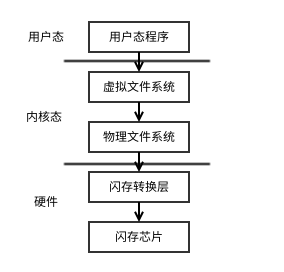
\includegraphics[width=0.4\textwidth]{traditional_ssd.png}}
    \hspace{4em}
    \subcaptionbox{开放通道SSD的访问流程\label{fig:imple_ocssd}}
        {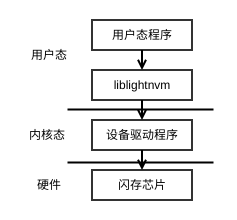
\includegraphics[width=0.4\textwidth]{ocssd.png}}
    \caption{两种SSD的访问流程}
    \label{fig:imple_ssdvisit}
\end{figure}

具体到本文的实现,由于可供评测的数据为高性能应用运行时文件系统下发的IO Trace,因此可以在用户态的评测程序中实现不同的优化策略,读取IO Trace进行重放并通过liblightnvm直接操作开放通道SSD。为了便于评测时统计相关信息,实现时没有直接使用liblightnvm提供的读写接口,而是在开源的开放通道SSD评测工具fox的基础上进行改进。fox在liblightnvm提供的接口基础上增加了统计信息的记录,能够测量全过程的平均吞吐量,读/写/擦除操作的平均延迟以及精确到每页的读/写/擦除操作的大小和延迟。fox本身只提供了几种预先定义的IO序列,用于测试开放通道SSD的连续读取、连续写入和读取写入按一定比例混合交替进行时的性能。利用这些序列可以得到所用SSD的基本性能如表\ref{tab:imple_ocssd_perf}所示:

\begin{table}[htb]
    \centering
    \begin{minipage}[t]{0.8\linewidth}
    \caption{开放通道SSD的基本性能}
    \label{tab:imple_ocssd_perf}
      \begin{tabularx}{\linewidth}{YY}
        \toprule[1.5pt]
        {\heiti 操作} & {\heiti 延迟(单位us)} \\\midrule[1pt]
        读一个Page & 101\\
        写一个Page & 116\\
        擦除一个Block & 434\\
        \bottomrule[1.5pt]
    \end{tabularx}
\end{minipage}
\end{table}

由表\ref{tab:imple_ocssd_perf}可知,SSD的基本操作中擦除耗时远远高于读、写耗时,因此为高性能应用负载设计合适的优化策略时,应尽量避免过多的擦除操作和多余的写入操作。位于用户态的负载优化策略同样需要实现传统SSD的闪存转换层具有的地址映射、垃圾回收和负载均衡功能。实际上为了提高性能,闪存转换层还需要设计IO调度,写缓存,故障恢复等机制,并在垃圾回收等环节使用多线程提高效率。但完整实现闪存转换层的所有功能工作量太大,限于时间和精力,这里的做法是在现有方法的基础上改进地址映射和垃圾回收方式,同时注意实现负载均衡,以探索目前的方法是否有优化空间。

\subsection{开放通道SSD的物理地址与内部结构的对应关系}
\label{imple:paddrmap}
\begin{figure}[H]
    \centering
    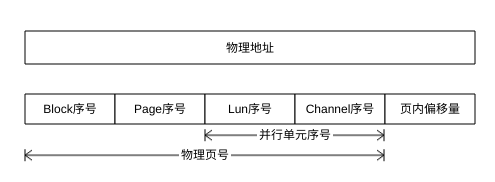
\includegraphics[width=0.8\textwidth]{paddrmap.png}
    \caption{开放通道SSD的物理地址与内部结构的对应关系}
    \label{fig:res_paddrmap}
\end{figure}
开放通道SSD按照如图\ref{fig:res_paddrmap}方式将物理地址编号与内部结构进行对应。一个用整形数表示的物理地址PA,从低位到高位各取若干位作为业内偏移量offset,Channel序号C,Lun序号L,Page序号P,Block序号B,则PA指向的开放通道SSD内部具体位置即为:第C个Channel的第L个Lun的第B个Block的第P个Page中从Page起始位置算起的第offset个Byte。将Lun和Channel放在地址的低位可以使连续的地址被分配到不同的Lun和Channel上,有利于利用设备内部的并行性。

页映射使用图\ref{fig:res_paddrmap}中Block序号、Page序号、Lun序号和Channel序号拼接得到每个物理页的唯一ID——物理页号。由于Lun和Channel的操作均相互独立,二者都被视为并行单元,为了对并行单元统一编号,使用图\ref{fig:res_paddrmap}中Lun序号和Channel序号拼接得到唯一的并行单元序号。

\section{优化策略设计}
由于目前开放通道SSD上开源的闪存转换层pblk采用页映射和贪心垃圾回收方式,并通过在各个Channel和Lun轮转选择写入和擦除块的方式实现负载均衡,故首先使用上述方式实现一个基本的优化策略,而后分别在映射方式和垃圾回收方面加以改进,同时保持原有的负载均衡机制。

\subsection{页映射-贪心垃圾回收策略(PM\_GCL)}
\subsubsection{重要结构描述}

\begin{table}[htb]
    \centering
    \begin{minipage}[t]{0.8\linewidth}
    \caption{页映射-贪心垃圾回收策略(PM\_GCL)重要结构描述}
    \label{tab:imple_pmstruct}
      \begin{tabularx}{\linewidth}{lX}
        \toprule[1.5pt]
        {\heiti 结构名称} & {\heiti 作用} \\\midrule[1pt]
        vpg2ppg & 页映射表\\
        ppg2vpg & 逆页映射表\\
        blk\_list & 每个并行单元上的块分配管理结构\\
        empty\_blks & 当前并行单元上的空闲块队列\\
        active\_blk & 当前并行单元上的活跃写入块\\
        non\_empty\_blks & 当前并行单元上已写满的块队列\\
        next\_ch\_lun\_i & 记录上次进行空间管理操作的并行单元序号的后继\\
        \bottomrule[1.5pt]
    \end{tabularx}
\end{minipage}
\end{table}

表\ref{tab:imple_pmstruct}描述了页映射-贪心垃圾回收策略用到的重要结构。

vpg2ppg为页映射表,用于完成逻辑页到物理页的映射。页映射方式的好处是映射关系较为灵活,缺点是页映射表的占用空间较大:设每个表项占用空间为$T$Byte,设备每个页容量为$P$Byte,则映射表所需空间为设备总容量的$T/P$。取$T=8, P=32768$,则映射表体积为整个设备容量的$1/4096$。当设备容量为4TB时,映射表所需内存高达1GB。页映射的另一个缺点是对映射表的更新操作较频繁,在进行覆盖写或垃圾回收操作时,物理位置发生变化的每个页的映射表项都需要更新。
ppg2vpg为逆页映射表,记录了每个物理页对应的逻辑页,用于标记物理页的分配状态,同时用于在垃圾回收过程中快速确定需重新写入的脏页对应的逻辑页号从而修改映射关系。

blk\_list为每个并行单元上用于分配单元内部块空间的管理结构。SSD设备的每个Channel和Lun的操作互相独立,均可视为一个并行单元。该结构通过2个队列和1个活跃块指针完成块空间的分配。empty\_blks用于管理当前单元内尚未被写入的块(空闲块),当需要分配空间时该结构将从空闲块队列上取下一个块,并将其设置为活跃写入块active\_blk用于放置对该单元的所有写入请求。活跃写入块写满后会被加入non\_empty\_blks队列等待垃圾回收。

为了最大程度利用设备的并行性,需要尽量使连续的逻辑页被分配到不同并行单元上。next\_ch\_lun\_i用于记录上次进行空间管理操作使用的并行单元序号的后继,用于使写入在不同单元之间进行轮转。

\subsubsection{映射方式}
\label{ssc:mapping}
\begin{figure}[H]
    \centering
    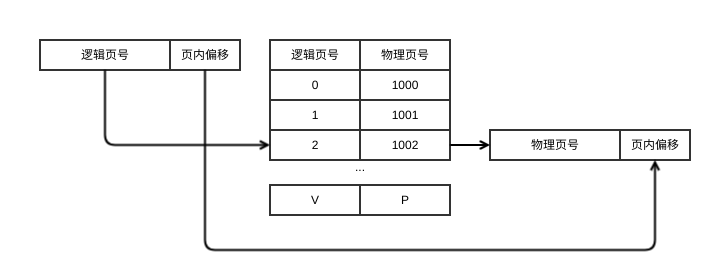
\includegraphics[width=0.8\textwidth]{page_mapping.png}
    \caption{页映射过程示意图}
    \label{fig:res_page_mapping}
\end{figure}

这一策略的映射方式使用页映射,映射过程如图\ref{fig:res_page_mapping}所示。逻辑页号由$\text{逻辑地址}/\text{页大小}$得到。物理页号由$\text{物理地址}/\text{页大小}$得到,对应图\ref{fig:res_paddrmap}中Block序号、Page序号、Lun序号和Channel序号共同组成的部分。对于传入的每个逻辑地址,策略通过查找页映射表将逻辑页号转换为物理页号,页内偏移量不进行改变,从而得到对应的物理地址。

对于写请求,策略总是需要为传入逻辑地址的逻辑页号分配新的物理页号:若当前逻辑页号尚未分配物理页号则显然需要;若已分配物理页号,则当前的写操作为覆盖写,需要将该物理页数据标记为无效,然后重新分配新的物理页存放覆盖写入的数据。分配新物理页号的过程如下:从next\_ch\_lun\_i开始遍历所有的并行单元,若遇到某个并行单元存在活跃写入块,或者不存在活跃写入块但存在空闲块则选择该单元进行空间分配。若所选单元没有活跃写入块则从空闲块队列中取出一个作为活跃写入块。若遍历所有并行单元后不存在符合条件的并行单元,则进行一次垃圾回收后重复遍历过程。遍历完成后,更新next\_ch\_lun\_i为当前选择单元的下一单元。最后,在所选的并行单元的活跃写入块中任意选择一个空闲页作为分配的新物理页,写入数据并更新页映射表和逆页映射表。

% 该过程中用到的主要接口如表\ref{tab:imple_pminf}:

\begin{table}[htb]
    \centering
    \begin{minipage}[t]{0.8\linewidth}
    \caption{页映射-贪心垃圾回收策略(PM\_GCL)映射过程主要接口}
    \label{tab:imple_pminf}
      \begin{tabularx}{\linewidth}{lX}
        \toprule[1.5pt]
        {\heiti 接口名称} & {\heiti 作用} \\\midrule[1pt]
        vpg2ppg(lm, vpg\_i) & 在映射表lm中查询,获取逻辑页号vpg\_i对应的物理页号\\
        ppg2vpg(lmr, ppg\_i) & 在映射表lmr中查询,获取物理页号ppg\_i对应的逻辑页号\\
        isalloc(lm, vpg\_i) & 查询逻辑页号vpg\_i是否已被分配物理页号\\
        allocate\_page(lm, vpg\_i) & 为逻辑页号vpg\_i分配物理页号,并维护映射表\\
        \bottomrule[1.5pt]
    \end{tabularx}
\end{minipage}
\end{table}

\subsubsection{垃圾回收}
垃圾回收过程中回收块的选择基于贪心策略:每次均选择所有已写满块中有效数据最少的一个块进行回收,在擦除的时间消耗一定时,贪心策略可以最小化重新写入脏页消耗的时间,同时最大化释放的空间。垃圾回收时机的选择遵循懒惰原则:当前写请求需要写入的数据量大于当前可用空闲页所能容纳的数据量时进行一次或多次垃圾回收,直到剩余空闲页能够容纳当前写入数据量为止。

垃圾回收的具体逻辑如下:首先从next\_ch\_lun\_i开始,遍历所有逻辑单元中的已写满的块队列,记录含脏页最少的块并选择为待回收块。遍历完成后更新next\_ch\_lun\_i为待回收块所在单元的后继单元。将待回收块内的所有脏页读入缓存并记录每个脏页所属的逻辑页号。将其移出该单元的已写满块队列,擦除该块,然后加入该单元的空闲块队列。对于读入的每个脏页,按照\ref{ssc:mapping}中的空间分配方式为其分配新的物理页,写入相应数据并更新映射表。由于被垃圾回收的任何块中脏页数量都小于该块的总页数,故每个脏页在原块被擦除成为空闲块后均能被分配新的物理页。

\subsubsection{负载均衡}
负载均衡主要通过以下2种机制实现:

物理页分配过程中,每次分配都会选择不同的并行单元上的活跃块空闲页,如此可以保证逻辑空间上连续的写入请求被均匀分布到不同的并行单元上,同时每个并行单元活跃块的选取遵循先进先出(FIFO)原则,刚刚被写满的活跃写入块只能加入写满块队列的尾部,等到其完成垃圾回收后又只能加入空闲块队列的尾部,在它第二次成为活跃写入块之前其他所有块都要完成一次擦除-写满的过程,因此不会出现同一个块被反复擦写而其他块不被访问的情况,故写负载在每个并行单元内也能够均匀分布到每个块上。

垃圾回收过程中,由于多个块同时具有最小脏页数量的情况时常出现,而垃圾回收算法总会选择其中第一个被访问的块,因此遍历时利用next\_ch\_lun\_i指针同样可以使得回收块的选择在不同并行单元上均匀分布。而物理页分配机制保证了每个单元中的块不会被短时间内多次写满,故擦除操作同样可以均匀分配到单元内的所有块上。


\subsection{页映射-连续空间垃圾回收策略(PM\_GCC)}
贪心垃圾回收需要为每个并行单元提供空间管理功能,结构略显复杂。一种可能的改进方式是模仿日志结构化文件系统(log-structured file system\cite{rosenblum_design_1992})的做法改进空间分配和垃圾回收方法。

\subsubsection{重要结构描述}
\begin{table}[htb]
    \centering
    \begin{minipage}[t]{0.8\linewidth}
    \caption{页映射-连续空间垃圾回收策略(PM\_GCC)重要结构描述}
    \label{tab:imple_lsstruct}
      \begin{tabularx}{\linewidth}{lX}
        \toprule[1.5pt]
        {\heiti 结构名称} & {\heiti 作用} \\\midrule[1pt]
        vpg2ppg & 页映射表\\
        ppg2vpg & 逆页映射表\\
        used\_begin\_ppg & 已写入区的起始物理地址\\
        used\_end\_ppg & 已写入区的结束物理地址\\
        \bottomrule[1.5pt]
    \end{tabularx}
\end{minipage}
\end{table}
表\ref{tab:imple_lsstruct}描述了该策略用到的重要结构。与页映射-贪心垃圾回收策略相比,该策略取消了对每个并行单元的空间管理,代之以划分设备空间为2个物理地址上连续的空间——已写入区和空闲区的做法。策略通过维护已写入区的起始物理地址used\_begin\_ppg和结束物理地址used\_end\_ppg(同时分别为空闲区的结束物理地址和起始物理地址)即可实现该功能。

\subsubsection{映射方式}
该策略的映射方式同样采用页映射,其地址转换机制与图\ref{fig:res_page_mapping}相同,接口形式与表\ref{tab:imple_pminf}相同,这里不再赘述。

初始状态下设备全部空间为空闲区。每次分配新的物理页时,设备将当前已写入区所在的结束物理地址指向的物理页分配出去,同时将该物理地址数值增加一个页的大小。根据\ref{imple:paddrmap}中的对应规则,增加后的物理地址将指向下一个并行单元的相同位置。这样对每个页的写入能够被分配到不同的并行单元上。
\subsubsection{垃圾回收}
该策略垃圾回收时机的选择同样基于懒惰原则:当空闲区的容量小于当前写入量时进行垃圾回收。在单次写入量小于Block容量的情况下,一次垃圾回收往往涉及对整个设备上所有块的访问。

垃圾回收时需要遍历整个已写入区,读出脏页和所属逻辑地址,擦除完成后重新写入并更新页映射表。遍历时为了利用并行性,同样遵循并行单元->Page->Block的遍历顺序,因此对Block的遍历并非逐个完成,而是一次完成并行单元数个Block的遍历,这要求用于存放脏页的缓存大小至少为并行单元数个Block大小。
\subsubsection{负载均衡}
从该策略的物理页分配方式可知,该策略将所有写操作均转换为对设备所有物理页的顺序写操作,因此写操作可以在所有页上均衡分布;在懒惰原则下和单次写入量不超过Block容量的情况下,一次垃圾回收会对设备的所有块进行擦除操作,故擦除操作同样能够均匀分布在所有块上。

\subsection{超级块映射-贪心垃圾回收方式(SBM\_GCL)}
另一种改进思路是增大映射的粒度。根据之前对高性能应用负载的分析,其IO Trace中存在大量的按页甚至按块对齐的覆盖写,因此在覆盖写过程中很可能出现整块的数据被标记为无效、需要回收的块完全不含脏页的情况。在这种情况下,逻辑地址与物理地址之间的映射往往是以块为单位进行的,采用粒度为块的映射完全可以在达到与页映射相同效果的同时大幅减少映射表占用空间和修改开销。
基于这一想法本文提出了超级块映射的改进方法,即将映射粒度从页增大到由一个或者多个块组成的超级块。
\subsubsection{重要结构描述}
\begin{table}[htb]
    \centering
    \begin{minipage}[t]{0.8\linewidth}
    \caption{超级块映射-贪心垃圾回收策略(SBM\_GCL)重要结构描述}
    \label{tab:imple_sbmstruct}
      \begin{tabularx}{\linewidth}{lX}
        \toprule[1.5pt]
        {\heiti 结构名称} & {\heiti 作用} \\\midrule[1pt]
        PN & 每个超级块包含的并行单元数\\
        BN & 每个超级块的每个并行单元包含的块数\\
        vsblk2psblk & 超级块映射表\\
        psblk2vsblk & 逆超级块映射表\\
        sblk\_list & 每个超并行单元上的超级块分配管理结构\\
        empty\_sblks & 当前超并行单元上的空闲超级块队列\\
        non\_empty\_sblks & 当前超并行单元上写入过的超级块队列\\
        next\_ch\_lun\_i & 记录上次进行空间管理操作的并行单元序号的后继\\
        \bottomrule[1.5pt]
    \end{tabularx}
\end{minipage}
\end{table}
表\ref{tab:imple_sbmstruct}描述了超级块映射-贪心垃圾回收策略所用的重要数据结构。

参数PN和BN定义了超级块的大小,每个超级块含有PN个并行单元,每个并行单元含有BN个块,故一个超级块含有$\mathrm{PN}\times \mathrm{BN}$个块。

该表中的其他结构与表\ref{tab:imple_pmstruct}中的结构大体相同,只不过将块替换为了超级块,同时由于每个超级块可能含有多个并行单元,故每PN个并行单元(称为一个超并行单元)分配一个超级块管理结构而不是每个并行单元都分配一个。一个区别是超级块映射中不需要为每个并行单元设置活跃写入块,non\_empty\_sblks队列不仅包含已被写满的超级块,也包含存在有效数据但尚未写满或者发生覆盖写的超级块。原因是在超级块映射下,一个超级块只要发生了覆盖写,即使该超级块尚未写满,其映射关系也需要更新,其中的所有数据被标记失效,所有脏页必须重新写入新超级块,随后该超级块中的脏页数量归零,随时可以进行垃圾回收。活跃写入块这种被写满后才可能被垃圾回收队列的机制在这里是不存在的。

\subsubsection{超级块地址结构}
超级块这一概念在开放通道SSD中并无实际物理结构对应,只是改变了块的组织方式,为了方便起见在此重新定义引入超级块后物理地址与开放通道SSD内部结构的对应关系。
\begin{figure}[H]
    \centering
    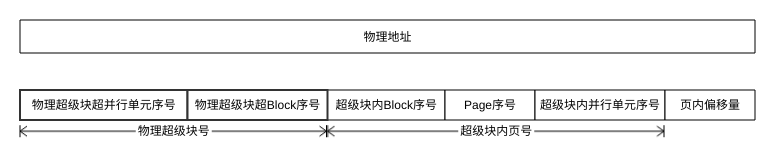
\includegraphics[width=0.8\textwidth]{sbaddrmapping.png}
    \caption{引入超级块概念后物理地址与开放通道SSD内部结构的对应关系}
    \label{fig:sbaddrmapping}
\end{figure}
对于一个Channel、Lun、Block、Page数分别为C、L、B、P的开放通道SSD,使用参数为PN、BN的超级块映射后物理地址与SSD内部结构的对应关系如图\ref{fig:sbaddrmapping}所示。一个物理地址PA可以从低位到高位依次划分为页内偏移量offset,超级块内并行单元序号inner\_pu,Page序号p,超级块内Block序号inner\_blk,物理超级块超Block序号outer\_blk,物理超级块超并行单元序号outer\_pu。该物理地址指向的SSD内部位置可按表\ref{tab:imple_sbaddrmapping}计算。在这种对应方式下,相邻的物理地址会对应到同一个超级块中,而在遍历同一个超级块内的地址时,遍历顺序仍然是按照并行单元->Page序号->Block序号进行的,即在同一个超级块内连续的物理地址仍然会分布在不同的并行单元上。
\begin{table}[htb]
    \centering
    \begin{minipage}[t]{0.8\linewidth}
    \caption{引入超级块概念后物理地址到开放通道SSD内部结构的转换方法}
    \label{tab:imple_sbaddrmapping}
      \begin{tabularx}{\linewidth}{lX}
        \toprule[1.5pt]
        {\heiti 参数} & {\heiti 值} \\\midrule[1pt]
        Channel 序号 & $(\mathrm{inner\_pu} + \mathrm{outer\_pu} \times (C \times L / PN))\mod C$\\
        Lun序号 & $(\mathrm{inner\_pu} + \mathrm{outer\_pu} \times (C \times L / PN)) \div C \mod L$\\
        Block序号 & $\mathrm{inner\_blk} + \mathrm{outer\_blk} \times (B / BN)$\\
        Page序号 & p\\
        页内偏移量 & $\mathrm{offset}$\\
        \bottomrule[1.5pt]
    \end{tabularx}
\end{minipage}
\end{table}

\subsubsection{映射方式}
\label{sssc:sbmapping}
\begin{figure}[H]
    \centering
    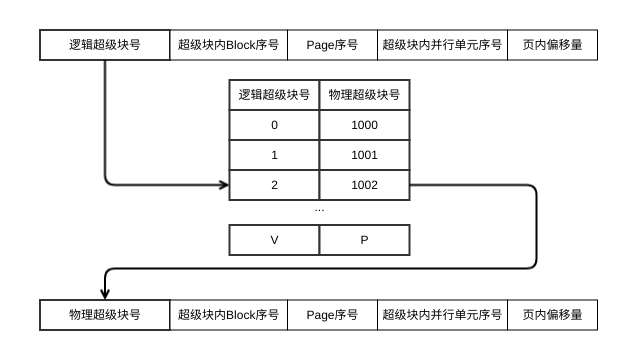
\includegraphics[width=0.8\textwidth]{sbmapping.png}
    \caption{超级块映射过程示意图}
    \label{fig:sbmapping}
\end{figure}
超级块映射与页映射的区别仅在于映射粒度,故图\ref{fig:sbmapping}中的地址映射过程与页映射类似。

对于写请求,该策略首先遍历写请求涉及到的逻辑页,尝试为每个逻辑页所在的逻辑超级块分配可用的物理超级块映射。若该逻辑超级块已经存在物理超级块映射,且逻辑页映射后的物理页可直接写入,则不改变映射关系;若该逻辑超级块不存在物理超级块映射或者存在映射但逻辑页对应的物理页为脏页,则需要为当前逻辑超级块分配新的物理超级块。分配流程与\ref{ssc:mapping}中分配物理页的过程类似:遍历所有超并行单元的分配管理结构,从空闲超级块队列中取出一个成员用于分配。若为写入脏页的情况,分配后除了写入当前写请求的数据和维护超级块映射表外,还要将原超级块的所有页标记为失效,并将其中未被覆盖写的脏页也写入新的超级块。

由于逻辑超级块和物理超级块是一一对应的关系,在不存在映射而进行分配的情况下策略必然能找到一个空闲超级块。但在待写入页为脏页而进行分配的情况下有可能出现无空闲超级块可用的情况,这时的处理方法有两种:一种是在读出未被覆盖写的脏页后直接擦除当前超级块,然后就地写入要写的数据和脏页;另一种方式是尝试进行垃圾回收,若回收得到超级块则继续按照分配成功的情况处理,若失败再回到第一种做法就地写入。第一种做法的优势是无需修改映射表,但由于映射表得不到更新,被擦除超级块的选择将完全取决于写请求访问的逻辑地址;第二种做法则更有利于负载均衡。

\subsubsection{垃圾回收}
由于引入超级块概念后物理地址与开放通道SSD内部结构的对应关系发生变化,连续空间垃圾回收方式中的已写入区和空闲区在引入超级块的对应方式下不再是物理地址上连续的区域,故采用超级块映射的优化策略无法使用连续空间垃圾回收,仍然采用基本优化策略的贪心垃圾回收方式。

垃圾回收的逻辑与页映射-贪心垃圾回收策略基本一致,区别仅在于将回收单位由块换成了超级块。一个简化的地方是由于超级块映射中需要回收的超级块内不存在脏页,故选择待回收超级块时可以直接选择脏页数为0的超级块而无需遍历所有待回收超级块获取脏页数量的最小值。

\subsubsection{负载均衡}
在贪心垃圾回收策略下,本优化策略具有与页映射-贪心垃圾回收策略相同的机制保证负载均衡。此外,\ref{sssc:sbmapping}中提到在写入页为脏页需要进行超级块分配但无空闲块可用时,先尝试垃圾回收后分配新超级块的方式与就地写入相比更有利于负载均衡,原因是该方式能够保持映射表的更新,使得相同的逻辑超级块地址多次访问时都能对应到不同的物理超级块地址,从而实现负载均衡。

% \section{映射方式}
% \subsection{直接地址映射}
% %直接地址映射即不进行任何形式的逻辑地址到物理地址的转换,这一策略最为简单,但不适用于SSD设备。原因是SSD设备的写入以Page为单位,而擦除以Block为单位,且被写入后的页只有在所在块被擦除后才能重新写入。当负载中存在大量的覆盖写时,

% \subsection{页映射}

% \subsection{超级块映射}

% \section{垃圾回收策略}
% \subsection{基于贪心原则的垃圾回收}
% \subsection{连续空间上的垃圾回收}

% \section{负载均衡}

\section{本章小结}
本章首先根据开放通道SSD访问特点确定了优化策略的实现层次,然后使用目前已有的开源闪存转换层pblk采用的地址映射、垃圾回收和负载均衡策略实现了最基本的优化策略。随后本章分别从垃圾回收算法和地址映射粒度两方面对基本策略尝试进行了改进,同时注意保持基本策略能够实现负载均衡的特点。